\documentclass[11pt]{article}

\usepackage[utf8]{inputenc}
\usepackage[T1]{fontenc}

\usepackage{amssymb,amsmath,amsthm,mathtools,mathabx,hyperref,txfonts,siunitx,booktabs,fontspec}


\hypersetup
	{ 
		colorlinks=true,       % false: boxed links; true: colored links
		linkcolor=blue,          % color of internal links (change box color with linkbordercolor)
		citecolor=green,        % color of links to bibliography
		filecolor=magenta,      % color of file links
		urlcolor=cyan,           % color of external links
		linkbordercolor	= {1 0 0},
		citebordercolor	= {0 1 0},	
		urlbordercolor	= {0 1 1}
	}

\newcommand{\definition}{\\ \textbf{Definition:} \hspace{1cm} }

\newcommand*{\QEDA}{\hfill\ensuremath{\blacksquare}}%
\newcommand*{\QEDB}{\hfill\ensuremath{\square}}%
\newcommand*{\ds}[1]{{\displaystyle #1}}
\newcommand*{\bild}{\begin{center} \textbf{BILD fehlt hier noch} \end{center}}

\begin{document}
	\title{Experimental Physik II Kapitel 19}
		\author
			{
				author\\
				{\small 	\texttt{email}}
			}
		\date{\today}
	\maketitle
	\tableofcontents
	\setcounter{section}{18} %Hier fängt die Nummerierung an.
	\newpage
	
	\section{Wellen}
	
	\begin{center}
	$ t=t_0 $:
\bild
Räumliche Periodizität

\rule{5cm}{.2pt}

$ \vec{r} = \vec{r}_0 $
\bild
zeitliche Periodizität
\end{center}

Welle: Zeitlich und räumlich periodische Auslenkung einer Zustandsänderung.\\
$ \Rightarrow $ Energie- und Impulstransport \underline{ohne} Materialtransport!\\
\paragraph{Experiment} \hfill \\
Einmalige Störung
\bild
$ \Rightarrow $ Kein periodischer Vorgang!

\paragraph{Experiment: WWW} \hfill \\
Periodische Erregung, Ausbreitung ohne Materialtransport!
\begin{itemize}
	\item punktförmiger Erreger: Kreiswellen
	\item linienförmiger Erreger: Ebene Welle
\end{itemize}
\paragraph{Heutz'sche Dipol} \hfill \\
Emission mit charakteristischer Abschallgeometrie
\paragraph{Verdichtungswelle ($ \Rightarrow $ "Wellenmaschine")} \hfill \\
$ \Rightarrow $ Unterschied: \underline{Transversalwelle}, \underline{Longitudinalwelle}

	\subsection{2 Arten von Wellenausbreitung}
\begin{itemize}
	\item Transversalwellen (Transversal Polarisiert) \\
	Schwingungsrichtung $ \perp $ Ausbreitungsrichtung\\
	z.B. Seilwelle:
	\bild
	\begin{center}
		
		2 Möglichkeitden der Polarisierung:
		\bild
		Transversalwellen sind polarisierbar
	\end{center}
	\item Longitudinalwellen (longitudinal Polarisiert)\\
	z.B. Schallwellen
	\bild
\end{itemize}

\underline{Mathematische Beschreibung der Wellenausbreitung}\break \\
"Störung" wandert mit Ausbreitungsgeschwindigkeit $ v_{Ph} $
\bild
\bild
Für mit-bewegten Beobachter bleibt Störung ortsfest (in \emph{S'})
$$ f(x')=f(x-v_{Ph}\cdot t) $$
$ \Rightarrow $ 1-dim Welle kann man beschreiben durch, $ \Psi(x,t) = \underline{\underline{f(x-v_{Ph} \cdot t)}} $ Jeder Punkt der Störung wandert mit $ v_{Ph} $ nach rechts. $$ v_{Ph} \text{: Phasengeschwindigkeit} $$
(Ausbreitung der Störung ohne Verformung!)\\
$ \Phi(x,t) $: Auslenkung, Druck, Dichte, $ \vec{E} $,$ \vec{B} $-Feld Amplitude, ...\\ \break
Sonderfall: Harmonische Wellen
\begin{align*}
\Psi(x,t) &= \Psi_0 \cdot \overbrace{\sin(K\cdot x -\omega t)}^{f(x,t)}\\
& \varphi = K \cdot x = \omega t \text{ : Phase}\\
K&: \text{Wellenzahl}\\
\omega&: \text{Kreisfrequenz}
\end{align*}
\hfill\\
\hypertarget{a}{(a)} \bild
\hypertarget{b}{(b)} \bild
\hyperlink{a}{(a)}
\begin{align*}
\Psi(x,t) = \Psi &= \Psi_0 \cdot \sin(Kx-\omega t)\\
&= \Psi_0 \cdot \sin(K(x+\lambda)-\omega t)\\
&= \Psi_0 \cdot \sin((Kx-\omega t)+K\cdot \lambda)\\
&\Rightarrow K \cdot \lambda = 2\pi &&\lambda \text{:Wellenlänge}\\
&\hspace{5mm} \Rightarrow K = \frac{2\pi}{\lambda}
\end{align*}
\hyperlink{a}{(a)}
\begin{align*}
\Psi &= \Psi_0 \cdot (Kx-\omega t)\\
&= \Psi_0 \cdot \sin(Kx-\omega (t+T))\\
&\Rightarrow\omega \cdot T = 2\pi \Rightarrow \omega = \frac{2\pi}{T} && \underline{T\text{: Periodendauer}}
\end{align*}

Wellen darstellbar:
\begin{align*}
\Psi(x,t) &= \Psi_0 \cdot \sin(Kx-\omega t)\\
&= \underline{\Psi_0 \cdot \sin (2\pi(\frac{x}{\lambda} - \frac{t}{T}))}
\end{align*}
In der Zeit \emph{T} (Periodendauer) breitet sich die Welle um eine Wellenlänge ($ \lambda $) aus.

$$ \Rightarrow \text{ Ausbreitungsgeschwindigketi } \boxed{ v_{Ph} = c = \frac{\lambda}{T} = \lambda \cdot \underset{\text{Frequenz}}{\nu} } $$

\begin{align*}
\Psi^{\pm}(x,t)&=\Psi_0 \cdot \sin(Kx\pm\omega t)\\
\Psi^{+} &\text{: läuft im Ortsraum nach links}\\
\Psi^{-} &\text{: läuft im Ortsraum nach rechts}
\end{align*}
	\subsection{Die Wellengleichung}

Erinnerung: Schwingungsgleichung: $ \ddot{\Psi} + \omega^2 \cdot \Psi = 0 $ \\
Lösung: Harmonische Schwingung: $  \Psi = \Psi_0 \cdot \sin(\omega t) $ \\
Wellen: Periodisch /bisher: auch harmonisch) in Ort und Zeit \\
\indent $ \Rightarrow $  Vermutung: Wellengleichung muss 2. Ableitung enthalten\\
Ansatz für $ \Psi $: $ \Psi(x,t) = \Psi_0 \cdot f(Kx-\omega t) $\\
$ f $ ist beliebig (aber periodische) Funktion der Phase $ \varphi $\\
$$ \frac{\partial\varphi}{\partial x} = K \hspace{5mm};\hspace{5mm} \frac{\partial\varphi}{\partial t} = -\omega$$
2. Ableitung berechnen:\\
Ort:
\begin{align*}
\frac{\partial\Psi}{\partial x} &= \Psi_0 \cdot \frac{\partial f}{\partial \varphi} \cdot \frac{\partial\varphi}{\partial x} && \text{(Kettenregel)} \\
&= \Psi_0 \cdot K \cdot \frac{\partial f}{\partial \varphi} \\
\hfill \\
\frac{\partial^2 \Psi}{\partial x^2} &= \Psi_0 \cdot K \cdot \frac{\partial^2 f}{\partial \varphi^2} \cdot \frac{\partial\varphi}{\partial x} = \Psi_0 \cdot K^2 \cdot \frac{\partial^2 f}{\partial \varphi^2}\\
&\Leftrightarrow {\color{CadetBlue}\underline{\Psi_0 \cdot \frac{\partial^2 f}{\partial \varphi^2} = K^{-2} \cdot \frac{\partial^2\Psi}{\partial x^2}}}
\end{align*}
Zeit:
\begin{align*}
\frac{\partial\Psi}{\partial t} &= \Psi_0 \cdot \frac{\partial f}{\partial\varphi} \frac{\partial\varphi}{\partial t} = -\omega \cdot \Psi_0 \frac{\partial f}{\partial\varphi}\\
\frac{\partial^2\Phi}{\partial t^2} &= \omega^2\cdot\Psi_0\cdot\frac{\partial^2f}{\partial \varphi^2} \Rightarrow {\color{CadetBlue}\underline{\Psi_0\cdot\frac{\partial^2 f}{\partial \varphi^2} = \omega^{-2} \cdot \frac{\partial^2\Psi}{\partial t^2}}}\\
\hfill \\
\Rightarrow &K^{-2} \cdot \frac{\partial^2\Psi}{\partial x^2} = \omega^{-2} \cdot \frac{\partial^2\Psi}{\partial t^2}\\
&\underline{\underline{\frac{\omega^2}{K^2} \cdot \frac{\partial^2\Psi}{\partial x^2} = \frac{\partial^2\Psi}{\partial t^2}}} &&\text{2. Ableitung nach Ort und Zeit verknüpft!!}
\end{align*}

mit $ v_{Ph} = \frac{\omega}{K} \hspace{5mm} \boxed{v^2_{Ph} \cdot \frac{\partial^2\Psi}{\partial x^2} = \frac{\partial^2\Psi}{\partial t^2}} $ ist die Wellengleichung in 1 Dimension! \\

$ f (x-v_{Ph} \cdot t) $ ist Lösung und beschreibt Ausbreitung in positiver x-Richtung!\\
Dann ist auch $ g(x+v_{Ph} \cdot t) $ Lösung, Ausbreitung in negativer x-Richtung!\\
\break
$ \Rightarrow $ Allgemeine Lösung der Wellengleichung:
$$ \Psi(x,t) = f(x-v\cdot t) + g(x+v\cdot t) $$
\begin{center}
	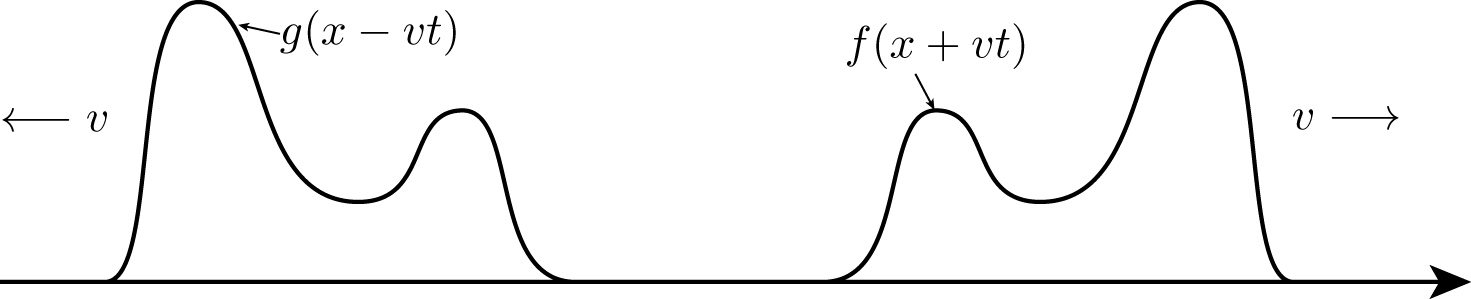
\includegraphics[width=0.7\linewidth]{skizzen/19/19B11}
\end{center}
\end{document}
